\chapter{Werkzeuge und technische Rahmenbedingungen}
\label{chap:tools}
Im folgenden Abschnitt werden einige wichtige technische Werkzeuge, die im späteren Verlauf eingesetzt werden, kurz und prägnant erläutert.
\begin{figure}[h]
	\centering
	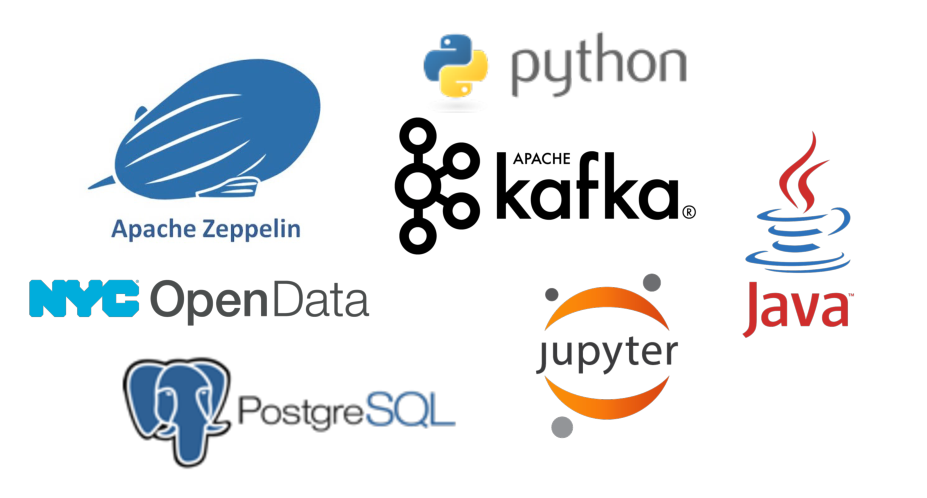
\includegraphics[width=7cm]{logos.pdf}
	\label{fig:logos}
\end{figure}

\begin{description}
	\item [Java] ist eine objektorientierte Open-Source Programmiersprache die ursprünglich von Sun Microsystems entwickelt wurde und heute zum Oracle Konzern gehört. In den letzten beiden Hauptversionen wurde der Sprachumfang  um funktionale und reaktive Aspekte erweitert. Java ist dank der \textit{Java Virtual Maschine} (JVM) als Laufzeitumgebung plattformunabhängig und hat sich vorwiegend in Enterprise Systemen und Web-Backends etabliert. Im Zuge der Verbreitung von BigData Projekten unter dem Dach der Apache Software Foundation, allem voran Hadoop und Spark, werden JVM sprachen wie Java und Scala nun auch im Bereich BigData eingesetzt.
	\item [Python] ist eine Open-Source Skripsprache, die sich hauptsächlich durch eine gut lesbare und knappe Syntax auszeichnet und unter anderem das objektorientierte und funktionale Programmierparadigma unterstützt. Im Gegensatz zu Java ist Python dynamisch typisiert und wird interpretiert anstatt kompiliert. Dank eines sehr umfangreichen und ausgereiften Ökosystems aus Frameworks und Bibliotheken zur Datenanalyse und maschinelles Lernen\footnote{z.B. TensorFlow von Google} ist Python im Bereich BigData  und dank der minimalinvasiven Eigenschaften zum Rapid Prototyping beliebt.
	\item [Apache Kafka] ist eine verteilte Data-Streaming Plattform der Apache Software Foundation, die ursprünglich von LinkedIn entworfen wurde. Beliebt ist Kafka im BigData Umfeld wegen seiner Skalierbarkeit und Fehlertoleranz.  Zu den Einsatzszenarien zählen vor allem Stream Processing, es kann aber auch als reiner Message Broker oder Speichersystem für Streaming Data verwendet werden. Die wesentlichen Komponenten von Kafka sind \textbf{\textit{Producer}} um einen Stream für einen \textbf{\textit{Topic}} zu veröffentlichen, \textbf{\textit{Kafka Cluster}} um die die Streaming-Daten verteilt pro \textit{Topic} im Dateisystem zu speichern und \textbf{\textit{Consumer}} um einen \textit{Topic} zu abonnieren und dessen Nachrichten zu lesen. Zudem können mit \textbf{\textit{Kafka Streams}} Nachrichten im Cluster transformiert werden. Mittels \textbf{\textit{Kafka Connectors}} kann man per Konfiguration gängige Datenquellen und -senken\footnote{wie z.B. Twitter oder JDBC} anschließen und stellen somit eine deklarative alternative zu den imperativen \textit{Producer API} und \textit{Consumer API} dar.
	2014 haben sich die verantwortlichen LinkedIn Mitarbeiter vom Mutterkonzern getrennt um sich mit der neu gegründeten Firma Confluent dediziert dem Apache Kafka Ökosystem zu widmen. Entwickelt wurde die quelloffene Software in der JVM-basierten Programmiersprache Scala, welche objektorientierte und funktionale Aspekte vereint.
	\begin{figure}[h]
		\centering
		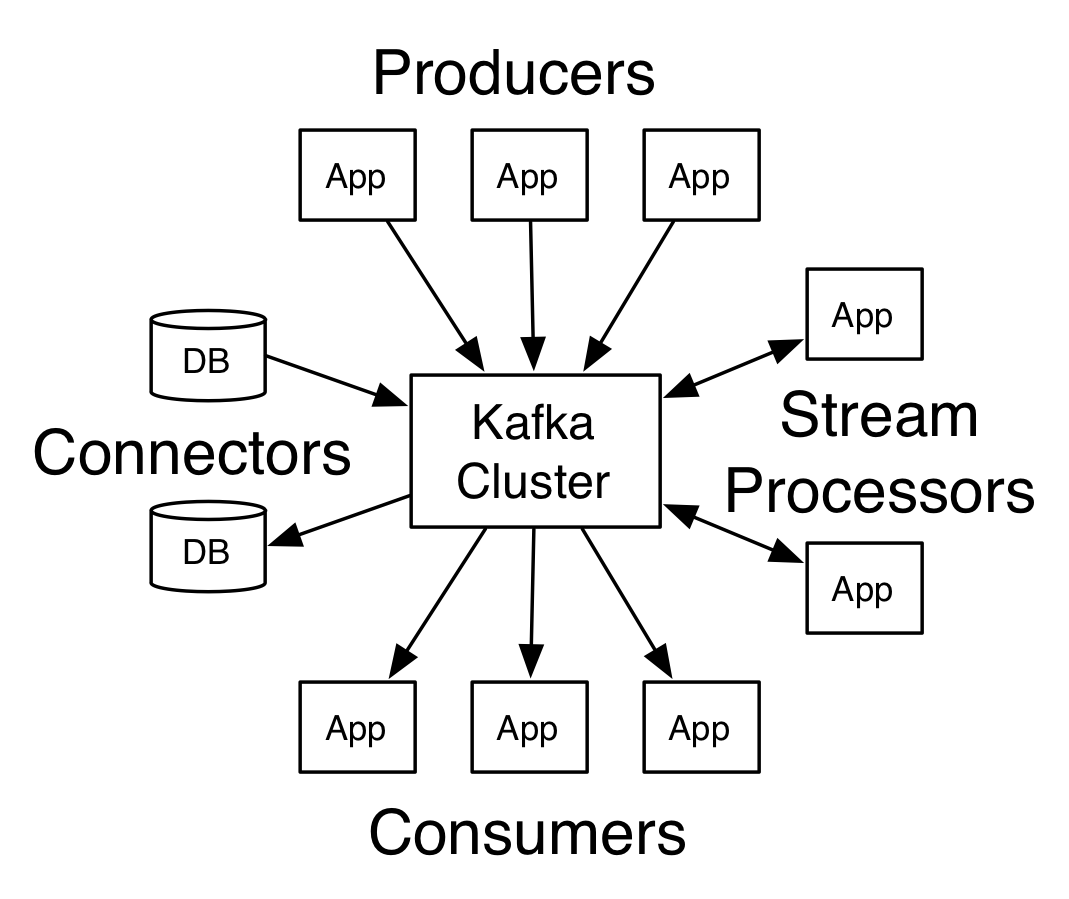
\includegraphics[width=7cm]{kafka-apis.png}
		\caption[Apache Kafka Architektur]{Apache Kafka Architektur\autocite{TODO}}
		\label{fig:KafkaArchitecture}
	\end{figure}
	\item [PostgreSQL] ist ein objektrelationales Datenbankmanagementsystem. Das vollständig ACID-konforme und in C geschriebene quelloffene System zeichnet sich durch einen breiten Funktionsumfang, Stabilität, Standardkonformität, hohe Erweiterbarkeit, und als Resultat dessen, eine weite Verbreitung aus. Neben dem traditionellen zeilenorientierten  Eigenschaften bietet PostgreSQL zudem Erweiterungen hinsichtlich verteilter, hoch-parallelisierter und  spaltenorientierter Datenverarbeitung, ein Geoinformationssystem sowie Volltextsuche. Auch im Bereich NoSQL bietet PostgreSQL eine dokumentenorientierter Speicherung und durch Erweiterungen sogar Graphen und Schlüssel-Werte-Datenstrukturen. Diese Flexibilität eröffnet PostgreSQL vielseitige Einsatzszenarien, darunter sowohl OLTP als auch OLAP.
	\item [Apache Zeppelin] ist eine Web-basierte Open-Source Software mit der man sog. Notebooks zur datengetriebenen, interaktiven und kollaborativen Analyse erstellen kann. Es werden eine Vielzahl an Speicher- und Analysetechnologien unterstützt, darunter SQL, Scala, Spark, Python und R. Im wesentlichen werden in einem Notebook polyglotte Abfrageskripte ad-hoc gegen die diversen Datenquellen ausgeführt und deren Ergebnisse in einem AngularJS, konfigurierbaren Web-Dashboard visuell und interaktiv dargestellt. Dadurch eignet es sich sowohl zur explorativen Datenanalyse als auch zum veröffentlichen und teilen von Analyseergebnissen.
	\item [Jupyter] ähnelt in den meisten Aspekten Apache Zeppelin, sodass sich alle oben zu Zeppelin genannten Punkte auch zu Jupyter nennen lassen. Die Unterschiede liegen eher im Detail der einzelnen Funktionen sowie der historisch und organisatorisch bedingten Nähe zu bestimmten Schlüsseltechnologien. Für das hier behandelte Forschungsprojekt spielen die individuellen Stärken und Schwächen der beiden Werkzeuge jedoch keine Rolle, weshalb beide Werkzeuge ebenbürtig eingesetzt werden.
	\item[\ac{SODA}] ist eine quelloffene Open Data Web-Programmierschnittstelle des U.S. Amerikanischen Dienstleisters Socrata. Anhand URLs werden Datasets adressiert und mittels der an SQL angelehnten \textit{Socrata Query Language} (SoQL) per HTTP GET in unterschiedlichen Datenformaten abgefragt. Zudem stehen SDKs für diverse Programmiersprachen zur Verfügung. Im Rahmen des Projektes werden wir die Datensätze der \ac{API} im \ac{JSON} Dateiformat abrufen.
	\begin{figure}[h]
		\centering
		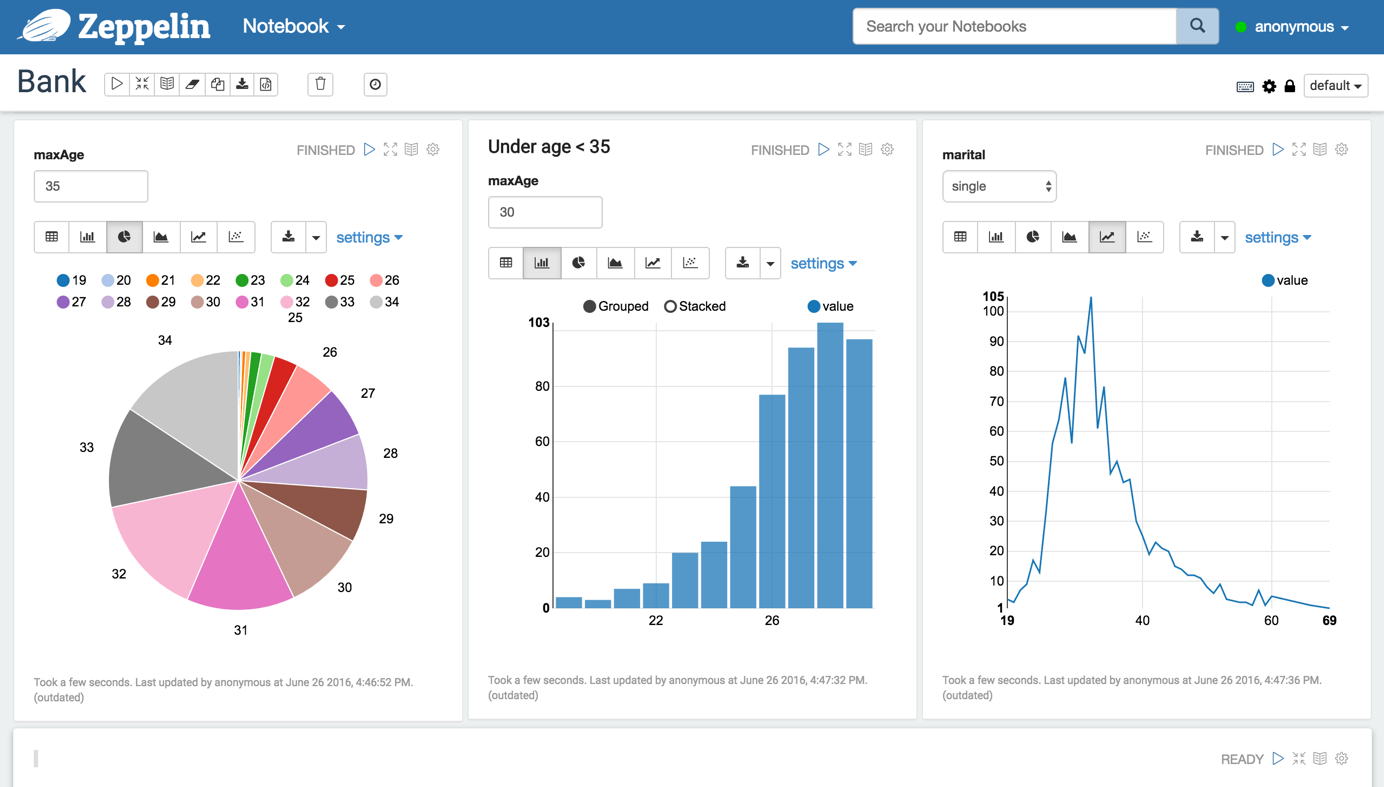
\includegraphics[width=\linewidth]{zeppeln_example_notebook.png}
		\caption[Beispielhaftes Notebook mit Apache Zeppelin]{Beispielhaftes Notebook mit Apache Zeppelin\autocite{TODO}}% https://zeppelin.apache.org/assets/themes/zeppelin/img/notebook.png
		\label{fig:zeppeln_example_notebook}
	\end{figure}
\end{description}
